% -------------------------------------------------------------------------------------------------
% QUALITATIVE EVALUATION
% -------------------------------------------------------------------------------------------------
\section{Qualitative Evaluation}
\label{sec:qualitative_evaluation}
In this section we will perform a qualitative evaluation of the developed work until the date. The
evaluation consists in compare the efficiency of the software stack required by our solution with
the other alternative solutions that are mentioned in the Related Work.

Another component that can be evaluated is the process to configure a smart place based on the
Fosstrak platform. In the standard solution there are two implemented clients that can be used to
configure the readers and events that belongs to a smart place. However, configure a smart place
with those clients is a manual process that is ineffective and error prone. In order to turn this
configuration process more automatic, our approach is to provide a client application that allows
the user to describe the smart place configuration in a JSON file, that later will be used by the
client to setup the readers and events in the application that is running in the Cloud.

\begin{figure}
  \centering
  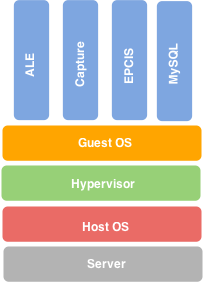
\includegraphics[width=.3\textwidth]{images/vm-stack}
\end{figure}
